% Main chapter 2:
\chapter{Theory}
\label{chap:theory}

\section{Recurrent Neural Networks}

Recurrent neural networks (RNNs) are optimal for processing sequential information. Some data are structured in a way in which the order of presentation is very important or parts of the problem can only be understood when having already seen previous information. Take the following sentence as an example: ``The dog barked at the cat'' has an entirely different meaning than ``The cat barked at the dog''. Another example would be weather data. If it rained the first 3 days and then got sunny for the rest of the week my prediction would be very different than if it was sunny the first 3 days and then started to rain. The RNN is able to process exactly that sequential component of the data. It extends a multilayer perceptron 
\cite{Rosenblatt58theperceptron:} by having recurrent connections within the hidden layers. This means that for every entry but the first in the sequence every neuron not only gets information from the new input but also from its previous timestep. A graphical demonstration can be found in figure \ref{fig:RNN}.

\begin{figure}[!htb]
	\centering
	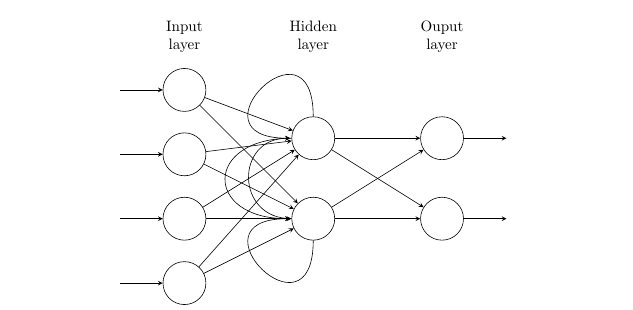
\includegraphics[width=0.7\textwidth]{images/RNN.png}
	\caption{Depiction of a recurrent neural network. Figure taken from \protect\footnotemark}
	\label{fig:RNN}
\end{figure}

The network can be unfolded over time to make the concepts easier to understand. For this the dimension is explicitly added. On the x-axis of figure \ref{fig:unfolded_RNN} 

\begin{figure}[!htb]
	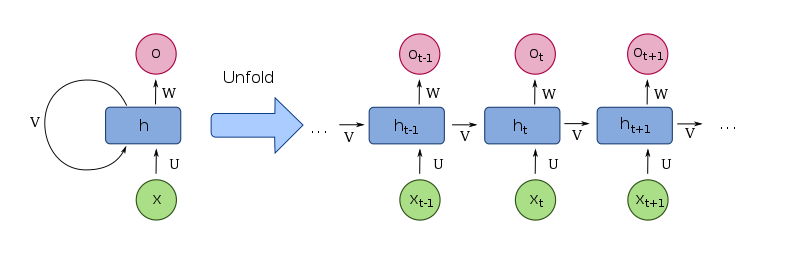
\includegraphics[width=0.9\textwidth]{images/unfolded_RNN.png}
	\caption{Depiction of a recurrent neural network unfolded over time. Figure taken from \protect\footnotemark}
	\label{fig:unfolded_RNN}
\end{figure}


\footnotetext{\url{https://tex.stackexchange.com/questions/364413/drawing-an-unfolded-recurrent-neural-network}}
\footnotetext{\url{https://en.wikipedia.org/wiki/File:Recurrent_neural_network_unfold.svg}}

the inputs are plotted in increasing chronological order. Now it is very clearly visible that the output of every cell is determined not only by its input at timestep $t$ but also from its own state at timestep $t-1$. \\
To train the network, backpropagation is modified to become backpropagation through time \cite{werbos_backpropagation_1990}, i.e. the gradient of the error is backpropagated through the network and the weights of the connections are adapted accordingly. 

\section{Vanishing Gradient Problem}

A problem with gradient-based learning is that the adaptions of the weights in early layers become vanishingly small when the number of layers becomes larger. This is due to the fact that the network weights are updated by the chain rule, i.e. they are updated proportional to the partial derivative of the error function with respect to the current weight. An example of the chainrule for the adaption of the weights to the output layer is given in equations \ref{eq:chain_rule_first} to \ref{eq:chain_rule_last}. $E, w_{ij}, o_j, v_j, \varphi$ are the error, weight, output of a neuron, weighted sum of inputs and activation function respectively.\\
When many layers are involved, the updates become exponentially smaller with an increasing number of layers between weight and output layer since the chain of derivatives gets increasingly longer. Given that for many sequential problems long sequences are used, backpropagation through time would either take incredibly long to train or not adapt weights for very early entries. To solve this problem long short-term memories were developed.


\begin{align}
	\frac{\partial E}{\partial w_{ij}} &= \frac{\partial E}{\partial o_j} \cdot \frac{\partial o_j}{\partial v_j} \cdot \frac{\partial v_j}{w_{ij}}
	\label{eq:chain_rule_first} \\
	\frac{\partial v_j}{\partial w_{ij}} &= \frac{\partial}{\partial w_{ij}}(\sum_{k = 1}^{n} w_{kj}o_k) = \frac{\partial}{\partial w_{ij}} w_{ij} o_i = o_i\\
	\frac{\partial o_j}{\partial v_j} &= \varphi'(v_j)
	\label{eq:chain_rule_last}
\end{align}




\section{Long Short-Term Memory (LSTM)}
\label{section:LSTM}

Long short-term memories (LSTMs) were developled in 1997 by Hochreiter and Schmidhuber \cite{LSTMHochreiter1997} to solve the vanishing gradient problem. An LSTM unit is composed of a cell with input gate, output gate and forget gate. The cell saves information over time like a buffer and the gates are used to control the flow of information in and out of the cell. A visualization can be seen in figure \ref{fig:LSTM}.

\begin{figure}[!htb]
	\centering
	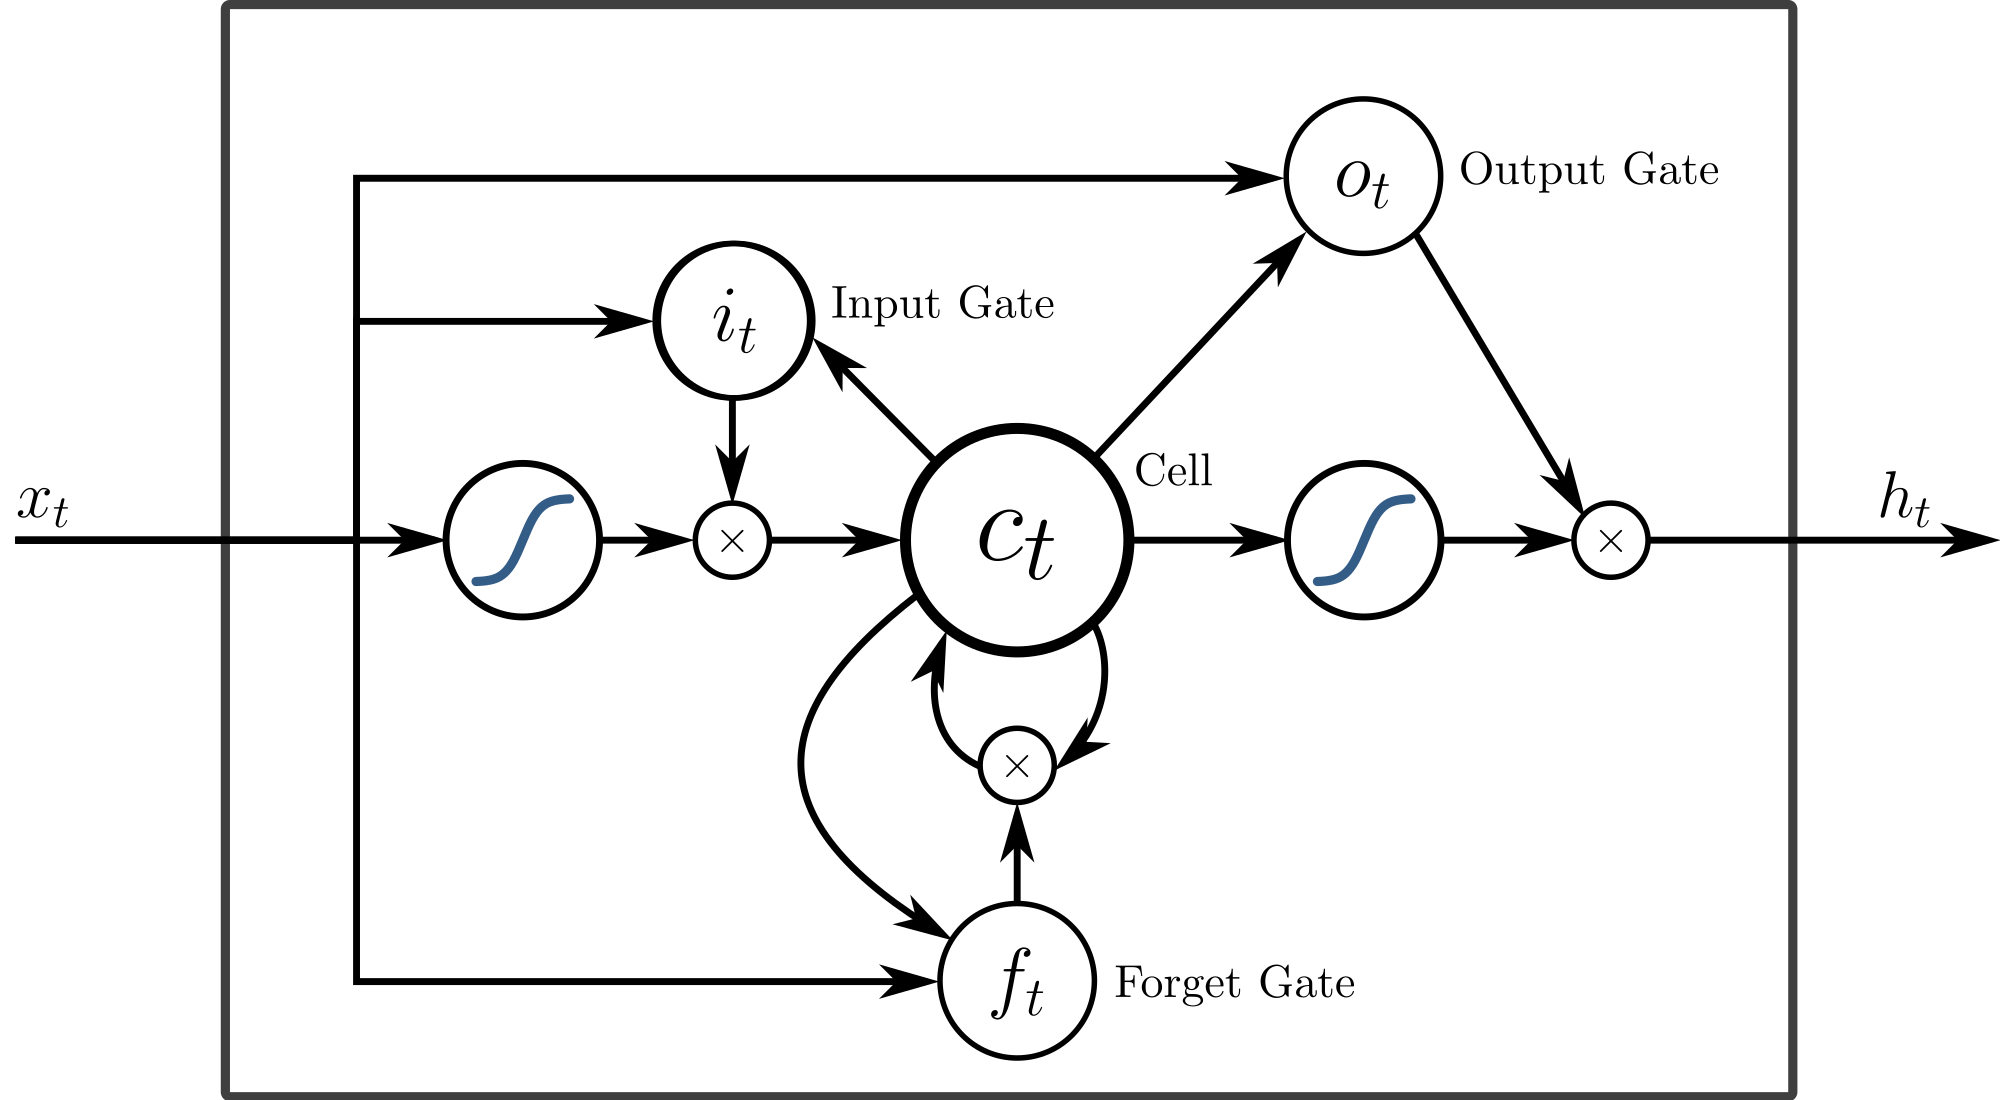
\includegraphics[width=\textwidth]{images/LSTM.png}
	\caption{visualization of an LSTM. Figure taken from \protect\footnotemark} 
	\label{fig:LSTM}
\end{figure}

\footnotetext{\url{https://en.wikipedia.org/wiki/Long_short-term_memory}}

The mathematical equations describing the functionality of the LSTM can be found in equations \ref{eq:LSTM_first} to \ref{eq:LSTM_last}, where $W_x$ and $U_x$ represent the weight matrices for the input and recurrent connections respectively and $b_x$ the biases. $x$ can be either $i$ for the input gate, $f$ for the forget gate or $o$ for the output gate. $c_0$ and $h_0$ are initialized with 0, $\circ$ denotes the element-wise multiplication of vectors and $\sigma$ is the logistic sigmoid function $\sigma(x) = \frac{1}{1 + \exp(-x)}$.

\begin{align}
	f_t &= \sigma_g(W_f x_t + U_f h_{t-1} + b_f) 
	\label{eq:LSTM_first}\\
	i_t &= \sigma_g(W_i x_t + U_i h_{t-1} + b_f) \\ 
	o_t &= \sigma_g(W_o x_t + U_o h_{t-1} + b_f) \\ 
	c_t &= f_t \circ c_{t-1} + i_t \circ \sigma_c (W_c x_t + U_c h_{t-1} + b_c) \\
	h_t &= o_t \circ \sigma_h (c_t)
	\label{eq:LSTM_last}
\end{align}


Importantly, the LSTM does not have the vanishing gradient problem, since it can store information over time intervals of arbitrary length. The experiments in this paper are therefore conducted with LSTMs. \\
A network can have multiple LSTMs in its hidden layer to process more complex information. The number of LSTM units per layer is called hidden size. Additionally, multiple LSTM units could also be combined sequentially. This is then called stacked LSTM. \\
In general, LSTM networks currently outperform most other architecture on sequential data and are also used for all experiments in this work. 

\section{Dynamic Time Warping (DTW)}
\label{section:DTW}

Dynamic time warping (DTW) is an algorithm designed to measure the distance between sequences that could vary in speed, frequency or other measures. If, for example, the similarity between two slightly shifted sinusoidal with the same frequency was to be determined, a standard approach, i.e. a mean squared error, might result in a numerically high difference even though the functions are very similar. To prevent this the DTW algorithm calculates the differences between the sequences for all values in the first sequence for every value in the second. This results in a 2D matrix of distances between the two sequences. To determine the distance a mean squared error is chosen. To find the DTW distance the path following the lowest costs starting at $(0,0)$ and ending at $(n,n)$ is chosen. The sum of the values along the path are the final result of dynamic time warping. An algorithm in pseudo code can be found in algorithm \ref{alg:DTW}


\begin{minipage}[right]{0.9\linewidth}
	\begin{algorithm}[H]
	\SetKwInOut{Input}{Input}
	\SetKwInOut{Output}{Output}
	
	\Input{\;
		$s_1:$ array[0..n],\; 
		$s_2:$ array[0..m]
		}
	\Output{\;
		DTW distance between $s_1$ and $d_2$}
	\underline{DTWDistance} $(s_1, s_2)$:\;
	\;
		DTW := array [n,m] 	(initialize array) \;
		\;
		DTW[0,:] := inf		(first column set to infinity) \;
		DTW[:,0] := inf		(first row set to infinity) \;
		DTW[0,0] := 0		(first value set to 0) \;
		\;
		\For{ i := 0 to n}{
			\For{j := 0 to m}{
				cost := d(s1[i], s2[j])		(calculate distance between points) \;
				DTW[i,j] := cost + min(DTW[i-1, j],    (insertion) \;
							DTW[i, j-1],   (deletion) \;
							DTW[i-1, j-1]) (match) \;
				}
			}
		\Return(DTW[n,m]))		
	\caption{dynamic time warping algorithm in pseudo code. $n,m$ represent the length of sequence 1 and 2.}
	\label{alg:DTW}
\end{algorithm}
\end{minipage}


Since the calculation requires taking the distance between all points for each point the resulting complexity is quadratic for sequences of the same length. To reduce computational complexity and therefore save time by not computing entries, that are likely irrelevant, in this paper the FastDTW algorithm was chosen. FastDTW has linear time complexity and comes at the cost of potentially slightly worse results. 

\section{Self-Organizing Feature Map (SOM)}
\label{section:SOM}

A self-organizing feature map (SOM) is used to produce low-dimensional (2D in this case) representations of the input space, usually called a map. A SOM is an artificial neural network that uses unsupervised learning and applies competitive learning instead of error-correction learning (like backpropagation) for the dimensionality reduction. Conceptually, a SOM unfolds the high-dimensional input space into a low-dimensional map, preserving the topological properties of the input, i.e. neighboring vectors in the input should also be neighbors in the output. \\ 
The map consists of multiple units to which weights are assigned at random in the beginning. After that a random vector is chosen from the training data and the best matching unit (BMU) of all weights is found, i.e. the unit with the smallest distance to the training sample. The neighborhood of the BMU is calculated. This means finding other units that are close to the BMU according to our chosen neighborhood function. After the neighborhood is determined the winning weight, i.e. the BMU is rewarded with becoming more like the sample vector. Neighboring units are also rewarded but to a lesser extend. In general, the higher the distance to the BMU the lower the reward for that weight. For this work a two dimensional Gaussian was chosen as the neighboring function. After repeating that process many times the average distance of every weight to their neighbors can be calculated and plotted. This is the easily visualized map that the SOM got its name from and which can be seen in multiple presentations of the experimental results in later sections. 

\section{k-Means Clustering}
\label{section:k-means_clustering}

The k-means clustering algorithm is used to find clusters of data points with high similarity in a given dataset. In this case the property to be compared is the Euclidean distance of the sequences. More specifically, the algorithm consists of two steps:\\
(1) Assignment: assign each data point to the cluster with the lowest euclidean distance to that point, i.e. the nearest mean of the cluster. \\
(2) Update: compute the new means to be the centers of the clusters. \\
If the assignments no longer change, the algorithm has converged. However, it is not necessary that the algorithm converges, since situations can arise in which the algorithm flip flops between two different states. Therefore the number of iterations in this paper is static and the final state needs to be taken as an approximation towards the real best state. In this paper the number of iterations was chosen to be high enough that SOMs for test samples did not change further. 